\chapter{Introduction}
\label{chapter:introduction}
    
    At the latest, since automated driving is gaining increased attention, it becomes clear that the automotive industry is not only about mechanics anymore.
    Information technology and computers play a big part in today's vehicles and are responsible for crucial tasks and controls.
    Today's vehicles consist of over 100 \acp{ECU}, as shown by Figure \ref{fig:ecu_network}, creating a big network of distributed hardware.
    A similar topology can be found in other distributed systems like data centers, where a variety of different, locally distributed hardware provides various services.
    However, data centers mostly do not provide the hardware separately or bind applications to specific servers.
    Instead, using a cloud middleware, the hardware and its resources are provisioned on-demand and independent from the actual hardware.
    With topics like image recognition, artificial intelligence, and data processing of, for example, sensor data, new requirements arise for automotive embedded hardware.
    Cloud Computing is already being used for similar tasks and is gaining popularity in general \cite{Holst2020, KPMG2020}.
    The current usage of Cloud Computing in the backend, the similarities between data centers and vehicle topologies, and the benefits of extending the backend cloud into the vehicle \cite{Weber2020}, suggest a great potential for an in-vehicle cloud.

    \vfill
    \begin{figure}[ht]
        \begin{center}
            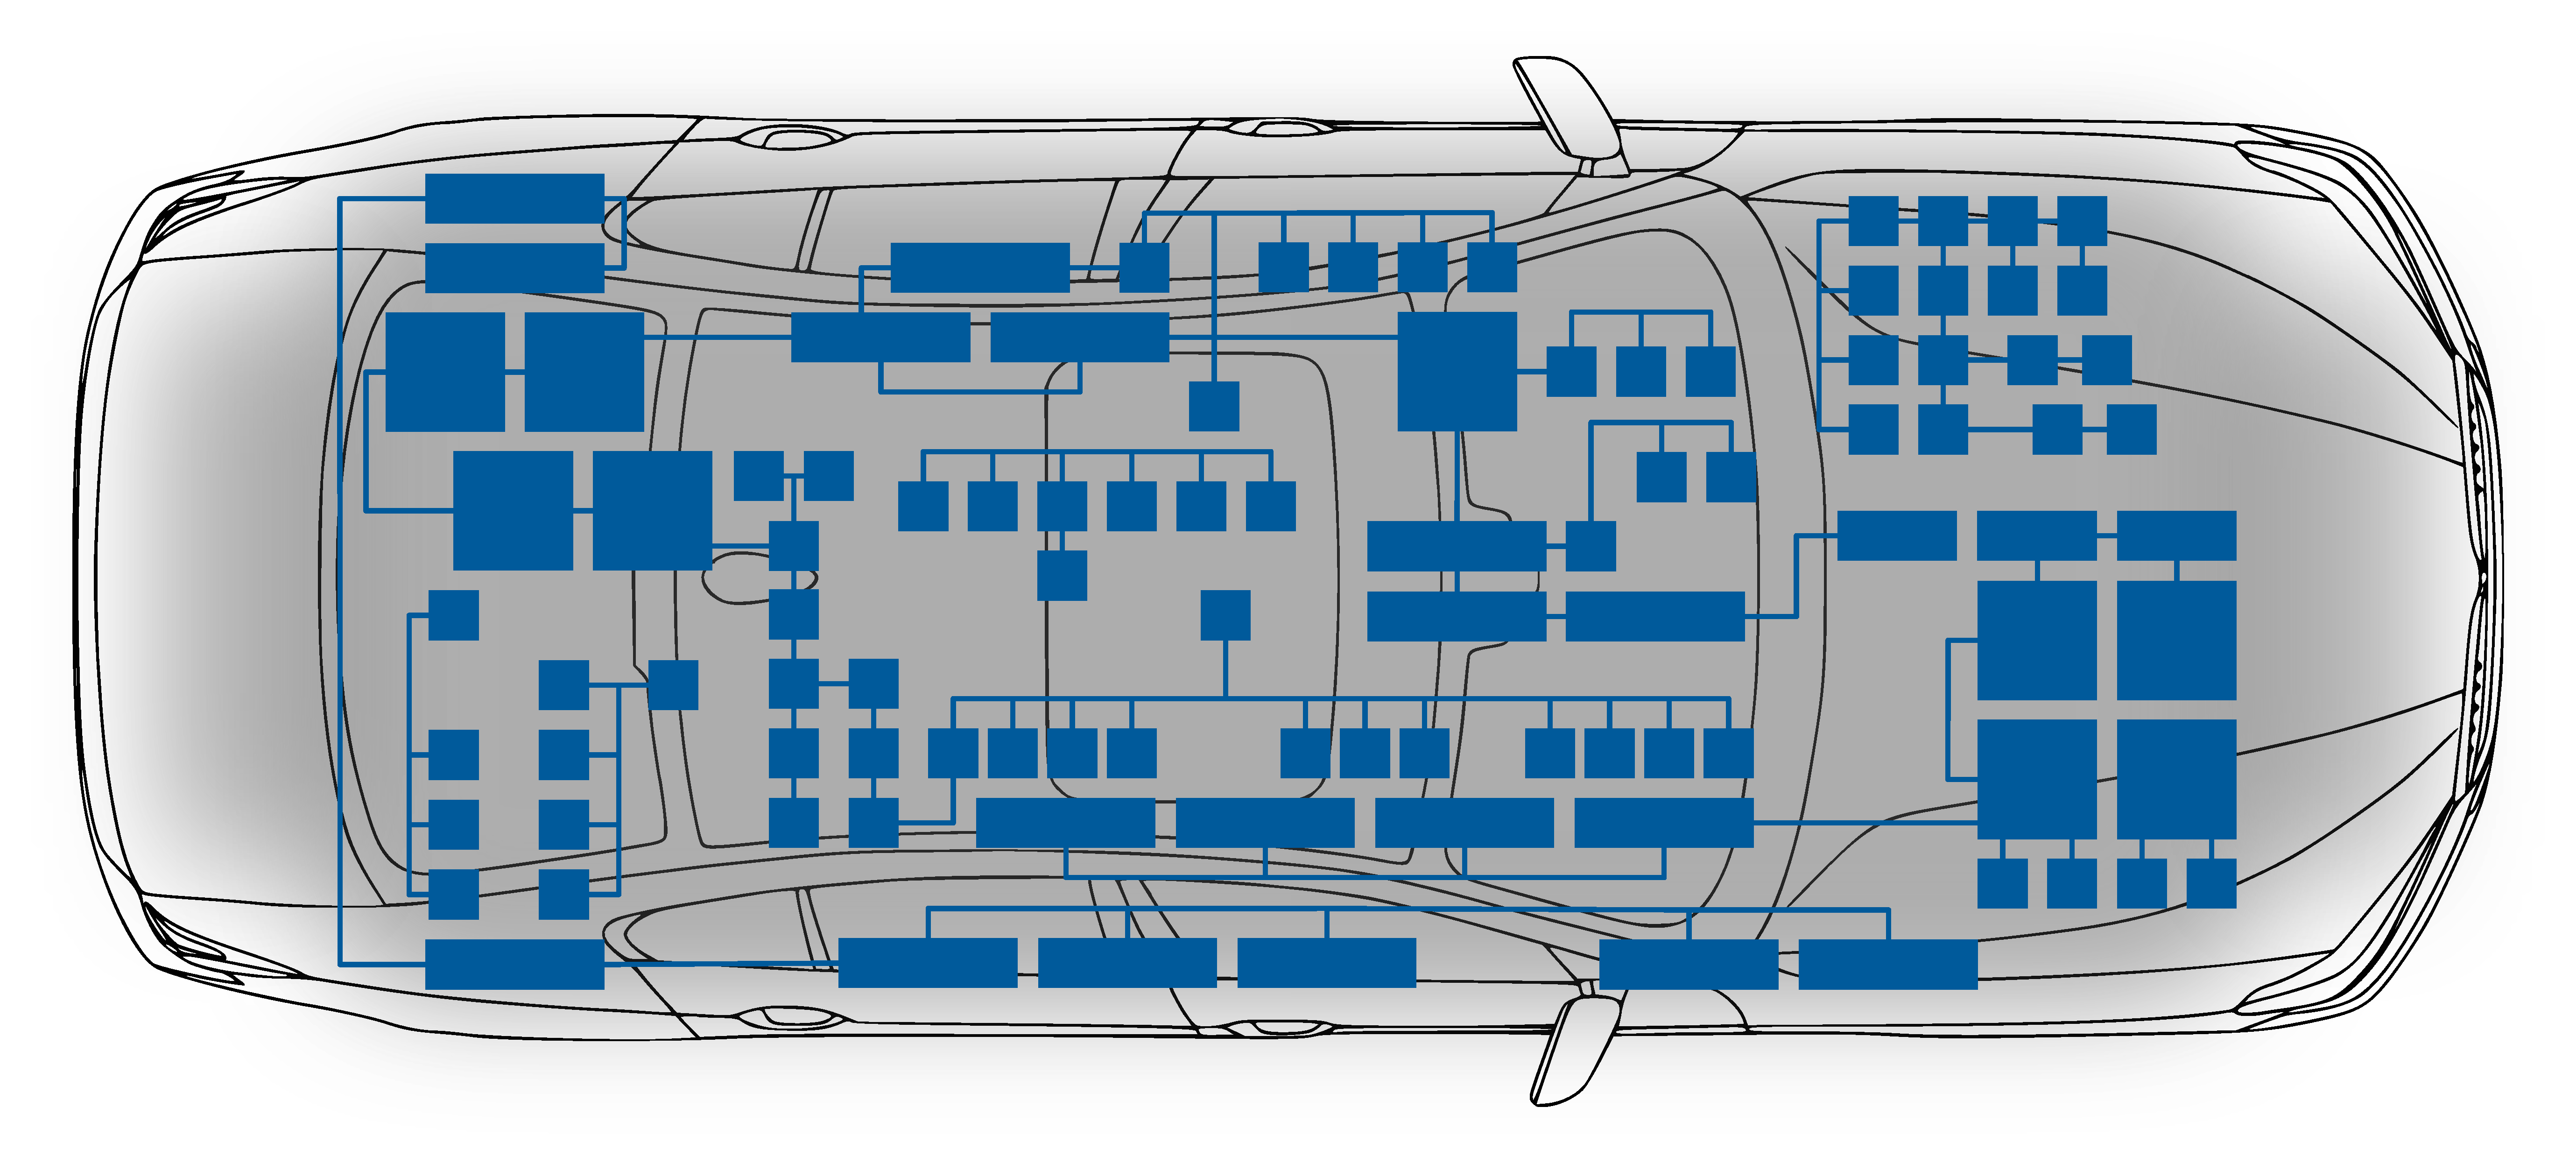
\includegraphics[width=0.9\linewidth]{01_ecu_network.pdf}
            \caption[Schematic ECU distribution in modern vehicles]{Schematic ECU distribution in modern vehicles according to \cite{Bosch2020,Drawingdatabase2020}}
            \label{fig:ecu_network}
        \end{center}
    \end{figure}
    \vfill
   
    
    %----------------------------------------------------------------------------------------
    %	Problem Definition
    %----------------------------------------------------------------------------------------
    \section{Problem Statement}
    \label{section:problem}
    
        \begin{center}
            \begin{minipage}{.9\textwidth}
                \textsl{"Cloud is about how you do computing, not where you do computing."}\\
                {\raggedleft \textsl{$\sim$Paul Maritz, CEO of VMware \cite{Nerdio2016}}\par}
            \end{minipage} 
        \end{center}
        
        \noindent In various disciplines and areas, the future is already  introducing unknown challenges.
        Challenges like autonomous driving or electric vehicles call for new approaches and require rethinking today's situation.
        The increasing demand for computational power and performance contradicts the embedded system characteristics, being very resource-aware and efficient.
        The rising number of \acp{ECU} installed in vehicles already exceeds 100 and makes their management nearly impossible, not even considering the software.
        Through various undertakings towards domain or vehicle centric E/E-Architectures \cite{Zerfowski2019}, the number of \acp{ECU} will decrease, however, multiple \acp{ECU} will still be present in a vehicle.
        Developing software for embedded systems requires engineers not only to solve tomorrow's challenges but also to face more restrictions and environmental factors than in most software development areas.
        Restrictions like cost, weight, or efficiency lead to highly optimized software at the expense of a challenging and complex development process and possibly abandoned functionality.
        
        \noindent To manage requirements and standardize automotive software development, Autosar plays an important role.
        Nevertheless, with the Autosar Classic documentation consisting of over 20.000 pages in the latest release, the standard's complexity is exploding.
        While Autosar enables the development of applications and functionality independently from the hardware, from a certain point, the software has to be statically assigned to specific hardware and, therefore, \acp{ECU}.
        As Paul Maritz said, today's challenges force us to concentrate on the problem itself and on the \textsl{how} we compute rather than concern ourselves with the \textsl{where} we compute.
        With the high number of \acp{ECU}, the rising software quantity and complexity, along with casual embedded system constraints and safety requirements, concentration on the \textsl{where} often shadows the \textsl{how}.
        
        \noindent Figure \ref{fig:ecu_pooling_today} depicts schematically how applications are currently assigned to particular \acp{ECU}.
        Cloud Computing already addresses these static assignations through a middleware representing separate, distributed systems as one pool of shared resources.
        Although Cloud Computing is used in many areas, including the automotive backend, it is yet to be used inside the vehicle.
        Using a middleware that virtualizes and provisions resources to \acp{VM} could facilitate the distribution of applications and software among multiple \acp{ECU}, as depicted by Figure \ref{fig:ecu_pooling_vision}, and overcome the static assignations.
        
        \begin{figure}[ht]
        \centering
            \begin{subfigure}[b]{0.45\textwidth}
                \centering
                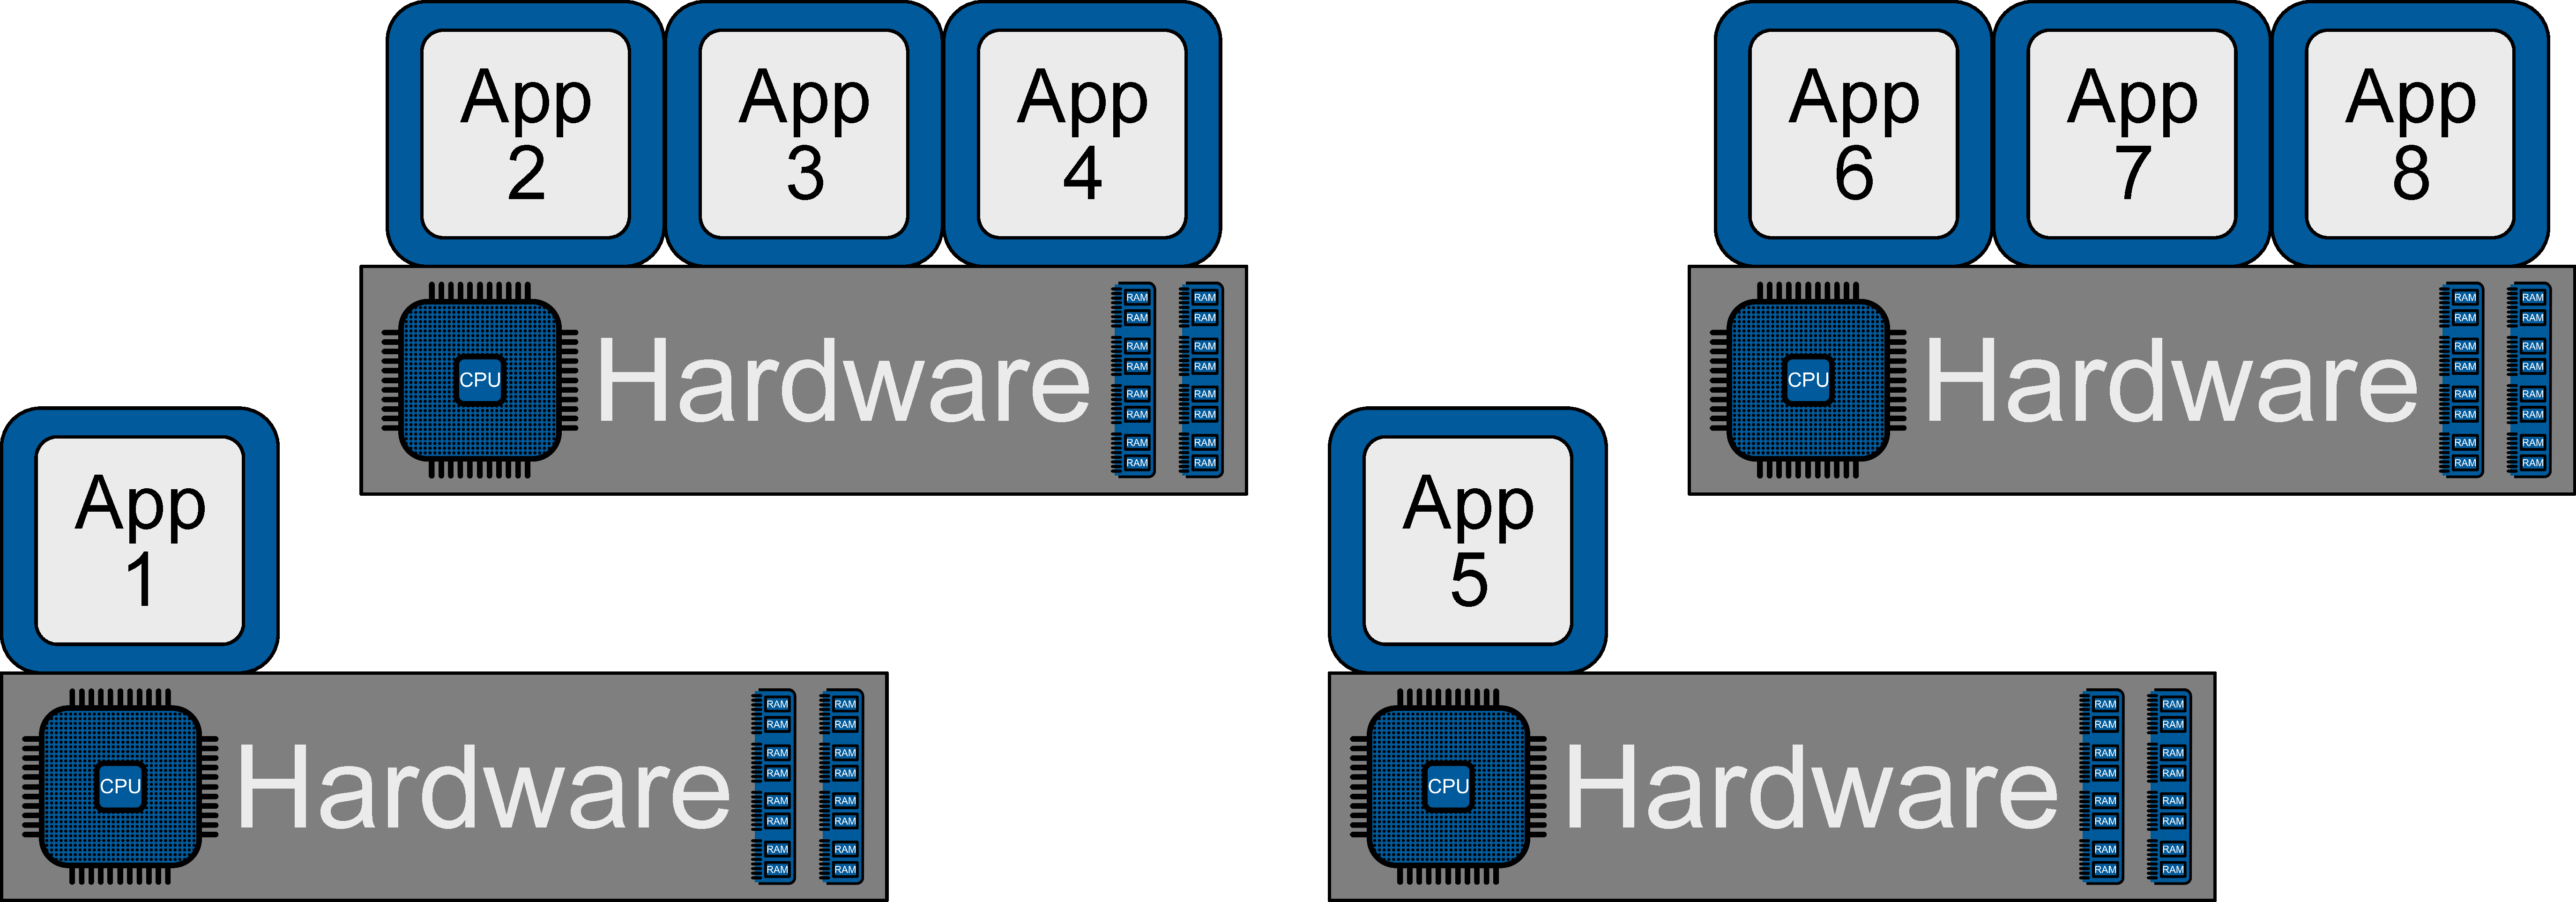
\includegraphics[width=\textwidth]{01_ecu_to_cloud_1.pdf}
                \caption{Today: Applications $\to$ Hardware}
                \label{fig:ecu_pooling_today}
            \end{subfigure}
            \hfill
            \begin{subfigure}[b]{0.45\textwidth}
                \centering
                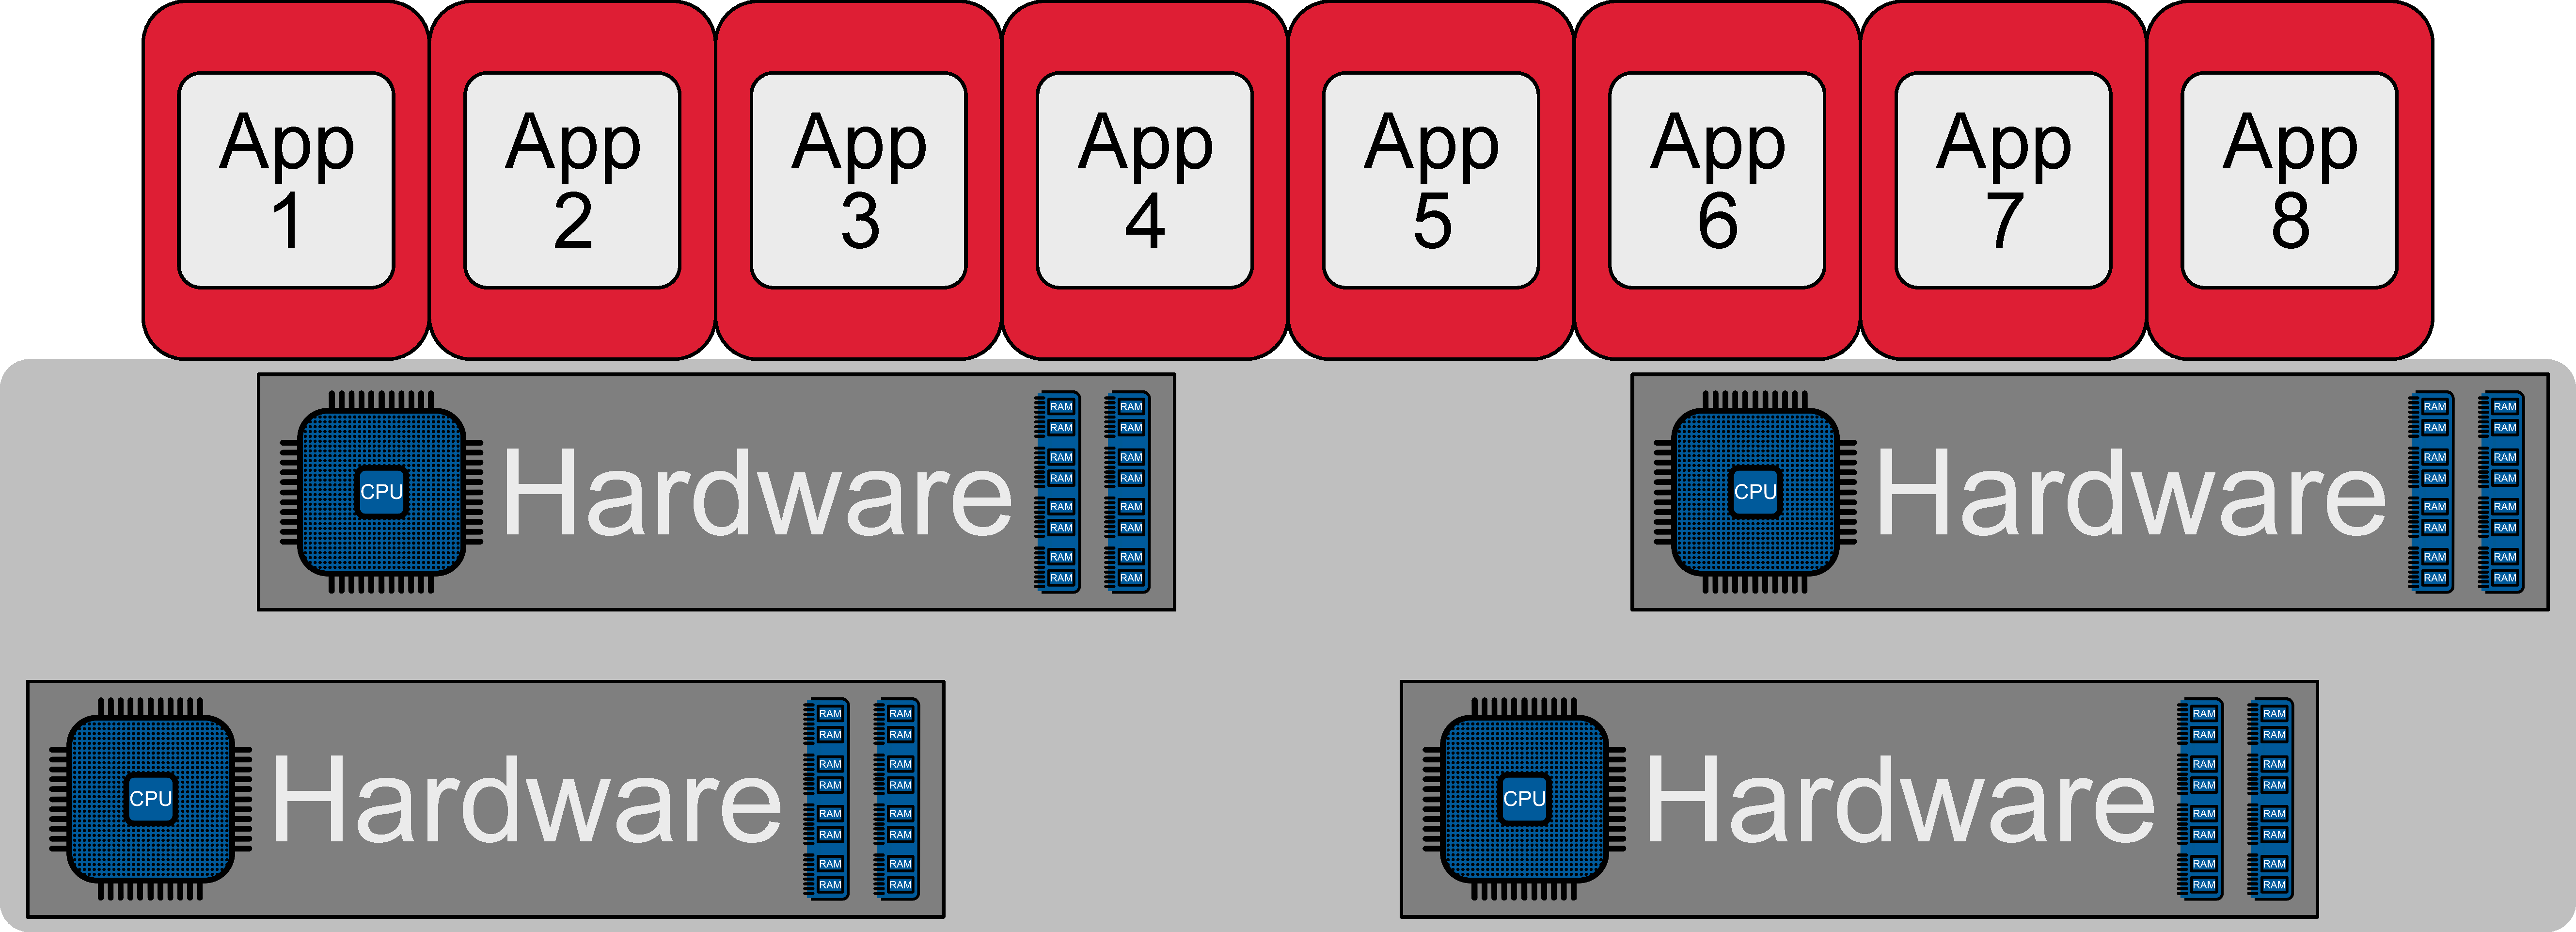
\includegraphics[width=\textwidth]{01_ecu_to_cloud_2.pdf}
                \caption{Vision: Applications $\to$ Shared Pool}
                \label{fig:ecu_pooling_vision}
            \end{subfigure}
            \caption{Symbolic depiction of distributed and pooled resources}
            \label{figure:ecu_pooling}
        \end{figure}

           
    %----------------------------------------------------------------------------------------
    %	Problem Definition
    %----------------------------------------------------------------------------------------
    \section{Goals and Research Question}
    \label{section:problem}
        
        \noindent Providers of Cloud Computing services like Amazon with Amazon Web Services or Microsoft with Microsoft Azure only provide the actual services.
        In contrast, the Open-Source project OpenStack \cite{OpenStack2021} aims at providing all the necessary tools and software to create an own cloud infrastructure.
        With OpenStack, one can deploy a cloud infrastructure on any hardware with sufficient resources.
        This thesis focuses on using OpenStack and its software components for providing computational resources on \acp{SoC} in embedded systems. 
        Therefore, the goal of the thesis presented shall be the successful execution of an OpenStack cluster on automotive embedded hardware.
        However, OpenStack's primary target hardware are servers in data centers.
        By consolidating different hardware into one OpenStack cluster, all resources can be pooled, represented as one shared pool, and provisioned to applications inside \acp{VM}.
        While embedded systems represent an area with specific requirements, OpenStack is developed for typical server environments.
        These contrasts and contradictions have an impact on the use of OpenStack on embedded systems.
        The extent of this impact shall be the research object of this thesis.
        Therefore, the main research question is:

        \begin{center}
            \textbf{Is it possible to leverage the advantages of Cloud Computing on embedded hardware?}
        \end{center}
        
        \noindent This question can be further divided into the following goals:
        \begin{enumerate}
            
            \item \textbf{Install and execute OpenStack on embedded automotive hardware.}\\
            As neither OpenStack is intended for embedded hardware, nor embedded hardware is intended for software like OpenStack, the installation has to be successful prior to actual evaluation.
            Due to custom \acp{OS} and kernels, as well as limited resources, the installation might pose difficulties.
            
            \item \textbf{Determine the impacts of Cloud Computing on embedded systems.}\\
            Due to neither working in the typical data center environment nor working with typical embedded software, special requirements and environmental constraints for OpenStack are present.
            It has to be determined how the contradictory requirements affect the embedded system and also OpenStack.
            On the other hand, it has to be determined whether and which Cloud Computing advantages can be leveraged on embedded systems.
            
            \item \textbf{Measure and evaluate identified impacts.}\\
            Having determined the positive and negative impacts of Cloud Computing, these have to be objectively quantified.
            To evaluate whether the impacts are substantial or negligible, measurements have to be performed in a defined way.
            
            \item \textbf{Evaluate OpenStack's performance on embedded hardware.}\\
            With impacts and their metrics defined, a cloud infrastructure on embedded hardware can be evaluated.
            Executing tests for the relevant metrics enables an assertion on OpenStack's performance on embedded hardware.

        \end{enumerate}
    
    
    %----------------------------------------------------------------------------------------
    %	Structure
    %----------------------------------------------------------------------------------------
    \section{Structure of this Thesis}
    \label{section:structure}
        
        The answer to the main research question is elaborated along the following structure:
        First, Chapter \ref{chapter:basics} establishes the basics in, for this thesis, relevant areas.
        Second, in Chapter \ref{chapter:host_and_Test_setup}, the preparation of the hardware used for the testing and the installation process of OpenStack itself is described.
        In Chapter \ref{chapter:methodology}, the test methodology for accessing OpenStack's overhead is presented, followed by the discussion of the results in Chapter \ref{chapter:measurements}.
        Chapter \ref{chapter:usecases} further examines two exemplary use cases as advantages of OpenStack, leading to a conclusion and outlook in Chapter \ref{chapter:conclusion}.

    
